\documentclass[11pt]{handout}
\usepackage{moreverb}
\usepackage{tabularx}
\usepackage{epsf}
\usepackage{epic}
\usepackage{eepic}
\usepackage{epsfig}
\usepackage{epsf}
\usepackage{fancyheadings}
\usepackage{fancybox}

\renewcommand{\coursetitle}{ECE 320}
\renewcommand{\handouttitle}{Surround Sound}
\renewcommand{\handoutauthor}{Swaroop Appadwedula}
\renewcommand{\semestertitle}{Spring 2000}

\newcommand{\bea}{\begin{eqnarray}}
\newcommand{\eea}{\end{eqnarray}}

\setlength{\parindent}{5mm}
\begin{document}

\setlength{\baselineskip}{0.5cm}
\setlength{\parskip}{0.5cm}

\makeboxtitle
\vspace{0.3cm}

\section{Introduction}
To begin understanding how to decode the Dolby Pro Logic Surround Sound 
standard, you will implement a Pro Logic encoder and a passive surround 
sound decoder.  This handout is only meant to give you an approach to 
tackling a surround sound project.  Significantly more technical 
information regarding Dolby Pro Logic can be found at \cite{Dressler}.

\section{Encoder}


%
%
% Module: surround_sound_matlab_exercise
%
% Author: Swaroop Appadwedula
%
%

In this section, you will implement the passive
encoder block diagram is shown in Figure \ref{fig:encoder} in \matlab.

\begin{figure}[htb]
    \begin{center}
	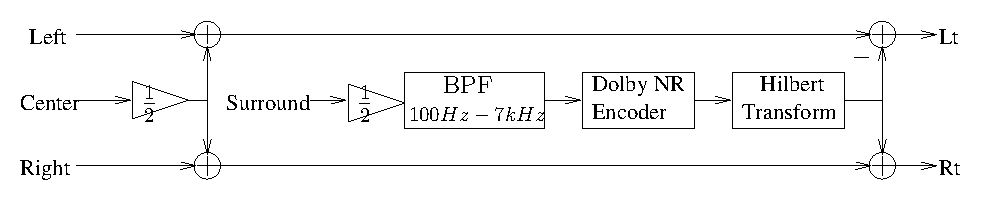
\epsfig{file=encoder.eps,width=13cm}
	\vspace*{0.5cm}
	\caption{Dolby Pro Logic Encoder}
	\label{fig:encoder}
    \end{center}
\end{figure}

The basic components of the encoder are multipliers, adders, a
Hilbert transform, a band-pass filter, and a Dolby Noise
Reduction encoder.  If you wish to implement Dolby Noise
Reduction, refer to \cite{Gundry}.  The other components are
discussed below.

The transfer function of the Hilbert Transform (HT) is shown in Figure
\ref{fig:hilbert}.  The transform is an all-pass filter with
a phase shift of $-90^{o}$.  Observe that a cosine input
becomes a sine and a sine input becomes a -cosine.  In \matlab,
generate a cosine and sine signal of some frequency and use the
\verb+hilbert+ function to do a HT of each signal.  The
imaginary part of the HT output (i.e \verb+imag(hilbert(signal))+)
will be the $-90^{o}$ phase-shifted version of the original signal.
Plot each signal to confirm your expectations.

\begin{figure}[htb]
    \begin{center}
	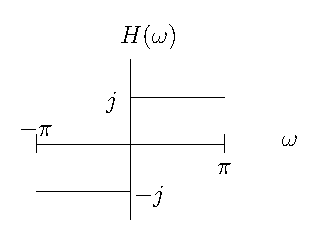
\epsfig{file=hilbert.eps,width=3.0cm}
	\vspace*{0.5cm}
	\caption{Hilbert transform transfer function}
	\label{fig:hilbert}
    \end{center}
\end{figure}

For the bandpass filter, design a second-order Butterworth filter
using the \verb+butter+ function in \matlab.

\paragraph{Generating a surround signal:}  Use simple mixing
techniques to generate a Pro Logic Surround signal.  For example,
use a voice signal for the center channel and fade a roaming sound
such as a helicopter from left to right and front to back.  In
\matlab, use the \verb+wavread+ and \verb+auread+ functions to
read \verb+.wav+ and \verb+.au+ audio files which can be found
on the Internet.




\section{Decoder}


%
%
% Module: surround_sound_processor_exercise
%
% Author: Swaroop Appadwedula
%
%

Implement the passive decoder shown in Figure \ref{fig:decoder} on
the DSP.  Use an appropriate time delay based on the distance
between the front and back speakers, and the speed of sound.

\begin{figure}[htb]
    \begin{center}
	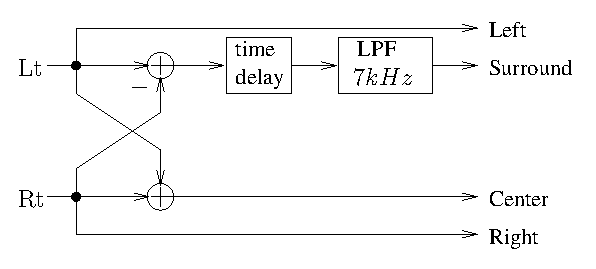
\epsfig{file=decoder.eps,width=8cm}
	\vspace*{0.5cm}
	\caption{Dolby Pro Logic Passive Decoder}
	\label{fig:decoder}
    \end{center}
\end{figure}

Is there significant crosstalk between the front and surround
speakers?  Do you get good separation between left and right
speakers?  How could power levels in the different channels be
used to provide directional enhancement?

For active decoding, you may consider using a Chamberlin filter
(see Chamberlin filter handout).  One way to find the power level
in a signal is to square it and pass it through a very narrow-band low-pass
filter ($\le 80 Hz$).
Squaring a signal in the time domain is equivalent to convolving
the signal with itself in the frequency domain.  In the frequency
domain, the resulting convolved signal near zero frequency corresponds
to the area under the original signal.



\small
\ifx\undefined\allcaps\def\allcaps#1{#1}\fi
\begin{thebibliography}{2}

\bibitem{Gundry}
K. Gundry, ``An Introduction to Noise Reduction,''
{\em http://www.dolby.com/ken/}.

\bibitem{Dressler}
R. Dressler, ``Dolby Prologic Surround Decoder Principles of Operation,''
{\em http://www.dolby.com/tech/whtppr.html}.

\end{thebibliography}

\end{document}

\bye 
